\documentclass[12pt,a4paper]{article}

\usepackage[T1]{fontenc}
\usepackage{lmodern}
\usepackage{wrapfig}
\usepackage{caption}

\usepackage{listings}
\lstdefinestyle{customc}{
  breaklines=true,
  frame=L,
  xleftmargin=\parindent,
  language=C,
  basicstyle=\footnotesize\ttfamily,
  keywordstyle=\bfseries\color{green!40!black},
  identifierstyle=\color{blue},
}

\usepackage{graphicx}
\graphicspath{ {images/} }

\usepackage{tikz}
\usetikzlibrary{arrows,positioning}

\usepackage[acronym]{glossaries}

\newcommand{\source}[1]{\vspace{-0.6cm}\caption*{Source: {#1}} }

\title{Video Game Control Panel}
\date{Last Updated: April 10th, 2017}
\author{Brett Mayson}

\tikzset{
    %Define standard arrow tip
    >=stealth',
    %Define style for boxes
    punkt/.style={
           rectangle,
           rounded corners,
           draw=black, very thick,
           text width=6.5em,
           minimum height=2em,
           text centered},
    % Define arrow style
    pil/.style={
           ->,
           thick,
           shorten <=2pt,
           shorten >=2pt,}
}

\makeglossaries

\begin{document}

\newacronym{PWM}{PWM}{Pulse with Modulation}
\newacronym{KSP}{KSP}{Kerbal Space Program}
\newacronym[plural=LEDs,longplural={Light Emitting Diodes}]{LED}{LED}{Light Emitting Diode}
\newacronym{RGB}{RGB}{Red, Green, Blue}
\newacronym{API}{API}{Application Program Interface}
\newacronym{LCD}{LCD}{Liquid Crystal Display}
\newacronym{TCP}{TCP}{Transmission Control Protocol}
\newacronym{HID}{HID}{Human Interface Device}
\newacronym{GCC}{GCC}{GNU Compiler Collection}

\pagenumbering{gobble}
\maketitle
\newpage
\tableofcontents
\newpage
\listoffigures
\printglossary[type=\acronymtype]
\newpage
\pagenumbering{arabic}

\linespread{1.5}

\section{Introduction}
\paragraph{}
This project's goal was to create a better gaming experience by creating a control panel for flight based games. It would be connected to a computer and used as a standard gamepad, allowing for compatibility with any game. Modifications would be created for some games to allow their data to be sent back to the gamepad to be displayed; this would set it aside from most similar projects, as almost all controllers are solely for input and most maker projects for video games focus only on output.
\section{Inspiration}
\paragraph{}
The inspiration for this project came from other makers who had created and shared their similar projects. Most of the projects I used for my inspiration had only targeted one game, mainly \gls{KSP}. The projects I saw mostly consisted of only outputs and displays, only a few featuring a small number of buttons. I wanted to take the information the previous makers had posted and use it to design a panel that consisted of both output and input and allow for the input to be used in any game.
\section{Design Process}
\subsection{Hardware}
\paragraph{}
The first step of the design process for the panel itself was finding a size to accommodate all the components originally planned. It needed to be large enough to comfortably hold all the parts without being too large to use conveniently on a desk in front of a monitor. In the end fancier displays like a \gls{LCD}, seven segment displays, and dials all had to be cut from the original plans for this project to fit everything onto the panel without sacrificing the final usability of the gamepad.
\paragraph{}
The construction of the enclosure was designed both for a wood based construction and 3D printed models. Wood was selected as the building material for its sturdiness, low cost and smaller construction time allowing for a higher margin of error. A 3D printed enclosure would take too long to reprint in the event of a design change or error in printing.
\newpage
\subsubsection{Input}
\begin{wrapfigure}{l}{0.3\textwidth}
	\vspace*{0cm}
	\centering
	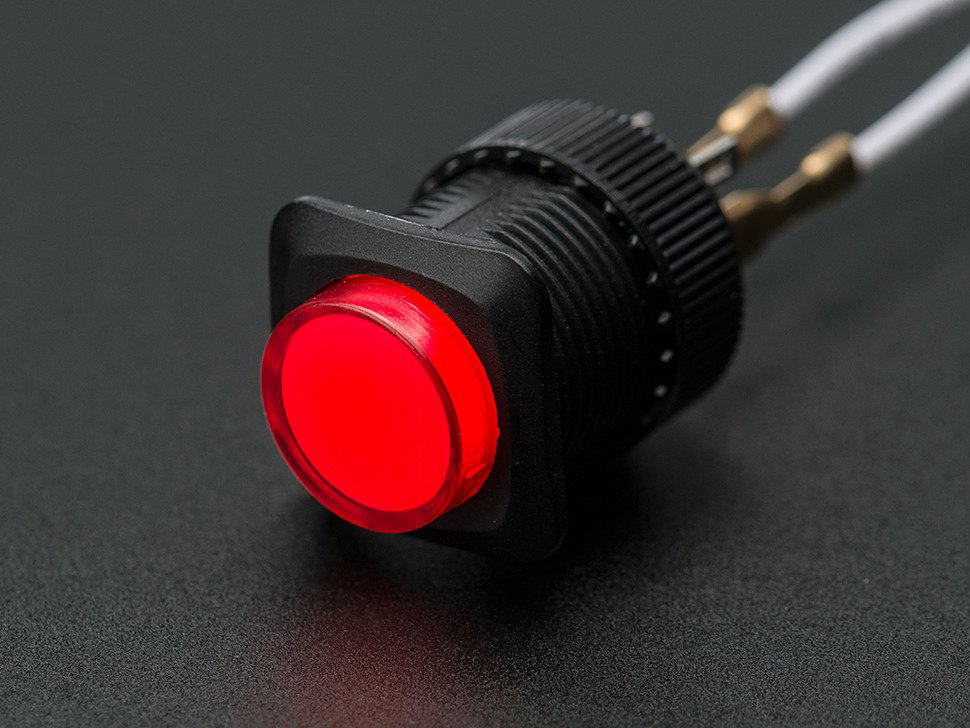
\includegraphics[width=0.3\textwidth]{button}
	\caption{LED Source}
	\source{Adafruit}
	\label{fig:button}
\end{wrapfigure}
\paragraph{}
The primary form of input on the control panel are 12 buttons. The buttons have built in \glspl{LED} (fig.~\ref{fig:button}) to create a clear sense of the status and severity of an action. If an action is dangerous and  permanent (separating boosters in a space game) then the button for that action would be flashing red. A safe action (for example looking at your map) would be a solid green button. This is to prevent accidental button pushes. If you are flying an airplane and want to view your map; you do not want to push the eject button accidentally.
\paragraph{}
\begin{wrapfigure}{r}{0.3\textwidth}
	\vspace{-0.2cm}
	\centering
	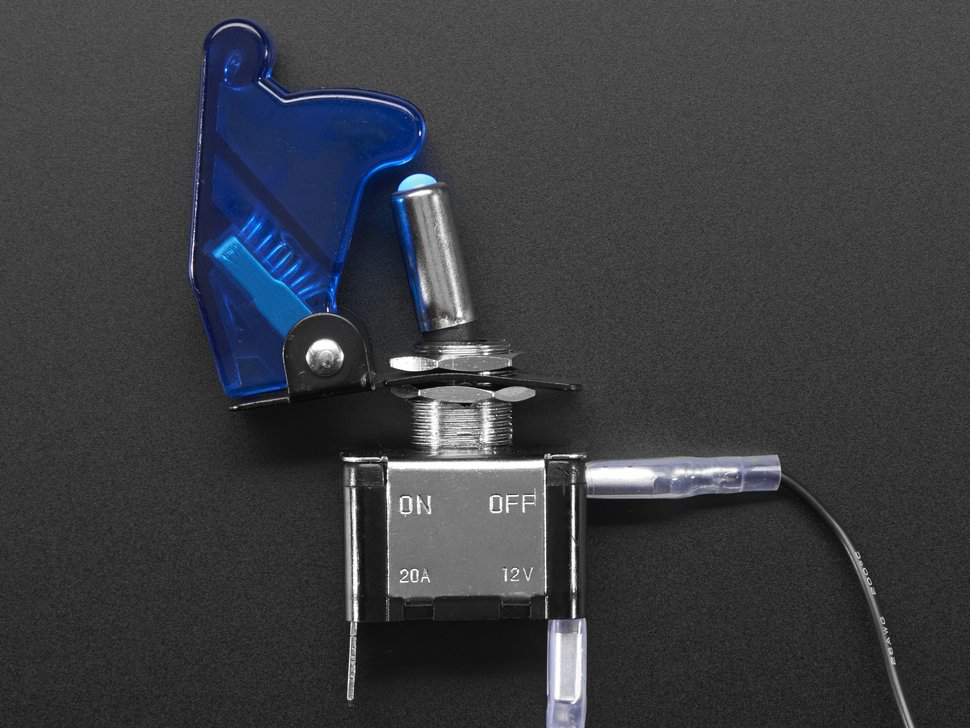
\includegraphics[width=0.3\textwidth]{toggle}
	\caption{Toggle}
	\source{Adafruit}
	\label{fig:toggle}
\end{wrapfigure}
Along side the buttons is a large toggle switch (fig.~\ref{fig:toggle}). The toggle switch is used to enable the use of the red buttons. When the switch is in the off position, the buttons are disabled in the Arduino's code, preventing their accidental usage before or after they are needed. Pushing the eject button, launching a spacecraft, disengaging primary engines and other potentially irreversible actions would all be mapped to these red buttons that require the toggle switch to be activated.

\subsubsection{RGB LEDs}
\paragraph{}
Unlike most gamepads which consist solely of inputs, \glspl{LED} were used to provide this control panel with output. \glspl{LED} are easy to understand and don't require time to read; they are fast and efficient for displaying the status of multiple components.
\paragraph{}
Every \gls{LED} on the panel is individually addressable and has \gls{PWM} capability.  Unlike standard \gls{PWM} which uses a 256 point scale (providing 16.8 million colors), the \gls{PWM} created for this panel uses a 32 point scale (32 thousand colors); this is to allow for a faster overall experience at the cost of accuracy of colors. The Arduino stores the \gls{PWM} value and then breaks down each cycle into 32 parts. If a \gls{LED} has a \gls{PWM} value of 16, it will be on for the first 16 cycles and off for the remaining 16; resulting in a half the brightness perceived by the human brain. Every \gls{LED} also has it is own state machine allowing the \glspl{LED} to act completely independent of each other. They can flash or fade at different rates, be linked to in-game information and have complete color control.
\paragraph{}
Along the top of the panel, a row of \gls{RGB} \glspl{LED} were placed. These allow for information to be displayed in a simple and concise manner. For example, in a space game, a \gls{LED} could be mapped to altitude changes. If your craft's altitude is not changing the \gls{LED} would be green, small changes in altitude would be yellow, larger changes would be red, and plummeting towards the surface would be flashing red. This system allows for quick recognition of problems that an \gls{LCD} is unable to provide. Multiple flashing red \glspl{LED} provide a much more obvious "something is wrong" indicator compared to numbers on displays.
\subsubsection{Joystick}
\paragraph{}
\begin{wrapfigure}{r}{0.35\textwidth}
	\vspace*{-1.5cm}
	\centering
	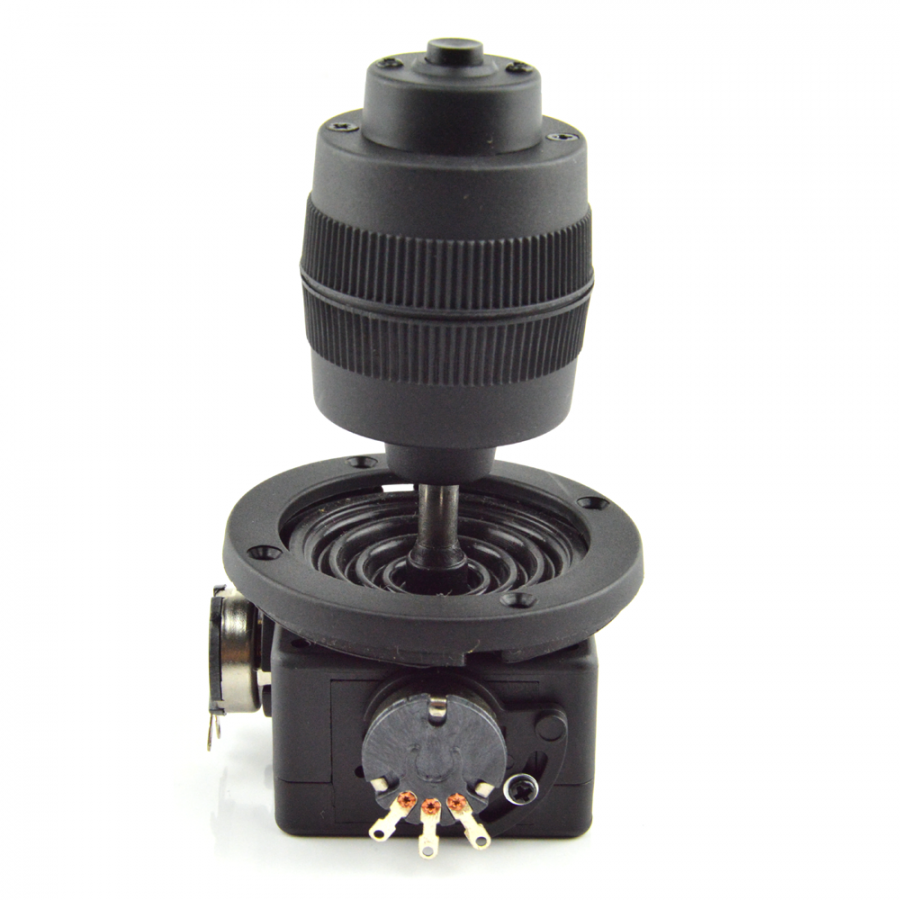
\includegraphics[width=0.35\textwidth]{joystick}
	\caption{Joystick}
	\source{RobotShop inc.}
	\label{fig:joystick}
\end{wrapfigure}
The control panel features a 3-axis joystick (fig.~\ref{fig:joystick}) with a single button located on the top. The joystick that was selected is small compared to many retail video game joysticks. The joystick only requires your thumb and index finger to use allowing for slow, fine movements. The primary purpose of the joystick is to control the docking procedure in \gls{KSP}, but it is compatible with any game that has support for a flight stick.
\subsection{Software}
\subsubsection{Arduino}
\paragraph{}
The code on the Arduino communicates with the computer software over an \gls{API} running on the serial connection. The Arduino responds to commands received over the serial connection. The commands are used to control the \glspl{LED} or any other output that may be added in the future. The Arduino is constantly sending the joystick's position to the computer to provide smooth motion in the game. Button commands are only sent when a button is pushed down or released. A status \gls{LED} on the Arduino lets the user see if a connection has been made to the software running on the computer and lets developers know when the Arduino is safe for flashing.
\subsubsection{Computer}
\paragraph{}
The software on the computer communicates with the Arduino over a serial connection. The software can send \gls{LED} commands and receives button and joystick information from the Arduino. These are then emulated on the computer as if the events came from a proper \gls{HID} joystick. The Arduino does not register on the computer as a \gls{HID} gamepad as that would not allow for information to be sent to the Arduino over a serial port, eliminating the ability to display in-game information on the panel.
\paragraph{}
The control software on the computer hosts a \gls{TCP} socket server allowing games with modifications installed to communicate with the software. The modifications for games are called sources. The sources collect information from the game and send commands to the control software. This allows the Arduino to display information from the game the user is playing. The source can also change key bindings for the software. Instead of the user mapping controls manually the source can tell the software what to make each button do.

\section{Build Process}
\paragraph{}
The bottom, front, and back of the panel are built from \(\frac{3}{4}\)  inch wood; the top of the panel with the components is made from thin particle board. The panel has 5x14 inches of usable space. Holes were drilled in the particle board for each component.
\newpage
\subsection{Hardware}
\subsubsection{Shift Registers}
\begin{figure}[!h]
	\centering
	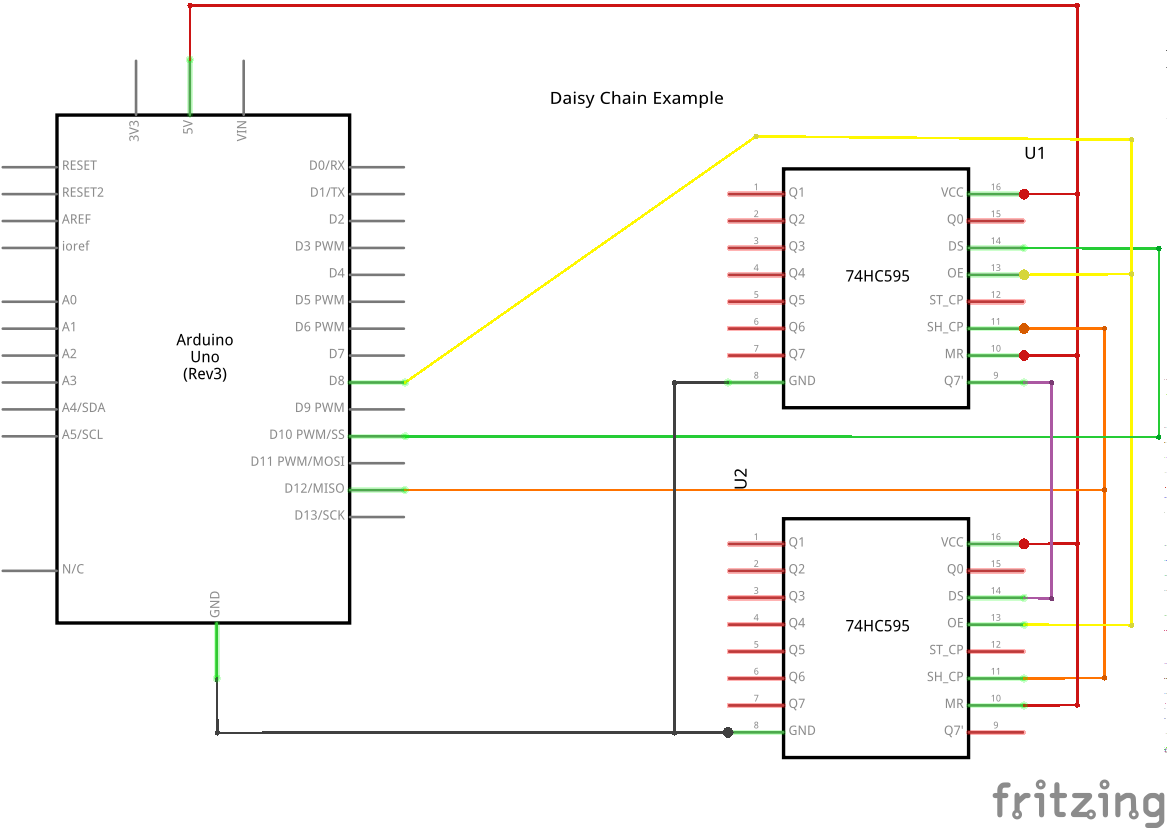
\includegraphics[width=0.8\textwidth]{daisy_chain}
	\caption{Shift Register Daisy Chain}
	\label{fig:daisy_chain}
\end{figure}
\paragraph{}
\begin{wrapfigure}[10]{r}{0.35\textwidth}
	\vspace*{-0.5cm}
	\centering
	\includegraphics[width=0.35\textwidth]{registers}
	\caption{Shift Registers}
	\label{fig:circuit}
\end{wrapfigure}
The most important component of the electrical circuit in the panel is the ten 8-bit shift registers. The registers are daisy chained together, essentially creating one 80-bit register. This is what allows this project to have so many digital inputs and outputs (fifty-six outputs \& fourteen inputs) even though the Arduino Uno used only has fourteen digital pins. There are ten unused pins on the shift registers allowing for future expansion. The panel only requires three outputs (data, clock, latch) and one input (buttons).

\subsubsection{Buttons}
\paragraph{}
The panel features twelve buttons and a toggle switch but only uses one digital input on the Arduino. This is accomplished by connecting the reference voltage of the buttons to the shift register instead of to a five volt source. Only one button is provided with a reference voltage at any given time; if the reference voltage is detected by the Arduino then the Arduino knows that button is pressed.
\subsection{Software}
\subsubsection{Arduino}
\paragraph{}
The Arduino software is programmed with C++ and uses the \gls{GCC} compiler as part of the Platformio ecosystem. Some non-standard C++ code is used and the \gls{GCC} or similar compiler is required. No makefile is provided and compiling with Platformio's tools is the best method.
\paragraph{}
The Arduino code is heavily dependent on the many state machines that have been created for each component type. These state machines allow all components to work independently of each other. The state machines tick in an order that allows the input to be recorded and sent to the computer without noticeable delay; the \glspl{LED} can flash fast enough that no flickering is visible.
\begin{figure}[h!]
	\caption{Example Loop Function}
	\lstset{escapechar=@,style=customc}
	\begin{lstlisting}
void loop()
{
  receiveCommands();
  if (connected)
  {
    sendJoystick();
    led.tick();
    in.tick();
    led.tick();
  }
}
	\end{lstlisting}
	\label{fig:fnc_loop}
\end{figure}

\subsubsection{Linux}
\paragraph{}
The control software for Linux is written in Python. Python was chosen as it allows quick development and testing as well as having a well documented Serial library. uinput, a kernel module for Linux, is used to emulate a joystick. python-uinput, a Pythonic library, is used to interface with the kernel module. The Python program receives joystick positions and button presses from the Arduino and then emulates those same actions on the computer.
\begin{figure}[h]
	\centering
	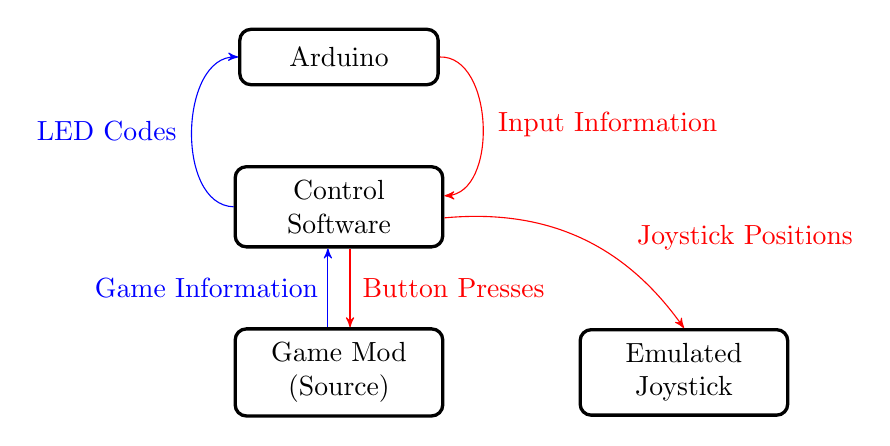
\begin{tikzpicture}[node distance=1cm, auto,]
		\node[punkt] (arduino) {Arduino};
		\node[punkt, inner sep=5pt,below=of arduino](software) {Control Software};
		\node[punkt, inner sep=5pt,below=of software] (source) {Game Mod (Source)};
		\node[punkt, inner sep=5pt,right=of source,xshift=20] (joystick) {Emulated Joystick};
		\draw[->,red]  (arduino.east) to[bend left=90] node[right,fill=white,xshift=2]{Input Information} ([yshift=4]software.east);
		\draw[<-,blue] (arduino.west) to[bend right=90] node[left,fill=white,xshift=-2]{LED Codes} (software.west);
		\draw[->,blue] ([xshift=-4]source.north) -- node[left,fill=white]{Game Information} ([xshift=-4]software.south) ;
		\draw[->,red]  ([xshift=4]software.south) -- node[right,fill=white,xshift=1] {Button Presses} ([xshift=4]source.north);
		\draw[->,red]  ([yshift=-4]software.east) to[bend left=30] node[right,fill=white,xshift=17] {Joystick Positions} (joystick.north);
	\end{tikzpicture}
	\label{fig:diagram}
	\caption{Flow Diagram}
\end{figure}
\subsubsection{Windows}
\paragraph{}
The control software for Windows is not functional at the time of this report. The software is being created using C++ and the vJoy device driver. vJoy is used to simulate a joystick when one is not available but the software being used requires one. The control software will use vJoy to turn the information from the Arduino into a simulated joystick.
\subsubsection{Game Modifications (Sources)}
\paragraph{}
Modifications for games that interact with the control software are called sources. They provide information that can be displayed on the panel's \glspl{LED} as well as tell the software how to map the buttons.
\paragraph{\gls{KSP}}
The \gls{KSP} source is written in C\#. The source sends spaceship status information to the control software to be displayed on the Arduino. It maps the buttons to actions based on their severity. The buttons are in three colors: red, blue and green. The \gls{KSP} source uses red for irreversible actions, blue for potentially irreversible and green for safe. The \gls{RGB} \glspl{LED} are used to display the status of various components as well as flight details.
\paragraph{Arma 3}
The Arma 3 source is written in C for the Linux version and C\# for Windows. Arma 3 is a military simulator with infantry, land vehicles and air vehicles. The source primarily focuses on helicopters although it can work on airplanes. The source uses the joystick to control the helicopter and uses the buttons to control doors, landing gear, trim and other aspects of the helicopter's flight. The \gls{RGB} \glspl{LED} are used to display the status of critical components and can flash or change color when a problem is detected. (Rotor damage, engine stall, etc.)
\paragraph{Future Sources}
The sources do not require any code changes to the control software or the Arduino. This allows any sources to be created in the future without a single change required to any of the existing code. The control software uses \gls{TCP} sockets to communicate with the sources allowing them to be written in any language that supports networking.
\section{Challenges}
\paragraph{}
The largest and re-occuring challenge while creating this project was the constraints of the Arduino Uno. Things like the low clock speed, limited digital pins, and slow, generalized functions had caused me to think about switching to a different microcontroller; but as I have a lot of experience with the Arduino I decided to find a solution that worked on it.
\paragraph{}
After deciding to use the same shift register from the course's labs (74HC595) I had some difficulty finding some; most of the code was tested on a single shift register even though the project required a minimum of nine. Once the shift registers had arrived and had been installed, my next challenge was getting the \gls{RGB} \glspl{LED} to work. \gls{RGB} \glspl{LED} require \gls{PWM} in order to display more than eight colors.
\section{Milestones}
\paragraph{}
A Major milestone for this project overcoming the limitations of the Arduino Uno. I was able to get all eighty inputs and outputs working through the ten shift registers. The speed of the \texttt{shiftOut} function was too slow and the \glspl{LED} were visibly flickering. Creating a faster way to output data to the shift registers was a huge accomplishment.
\paragraph{}
I am very happy with how the structure for the code turned out. Everything is abstracted to libraries allowing for a clean and clear sense of flow in the main logic of the program (fig.~\ref{fig:fnc_loop}). The way the game modifications have been designed allows for more to be created in the future with very little worry of limitations in the Arduino code or control software.
\section{Conclusion}
\paragraph{}
This project has resulted in a gameplay experience that is more satisfying and versatile than a standard gamepad and meets the goals it originally set out to accomplish. The project is not hard to expand, the shift registers have ten unused pins and the code is fast and efficient, so more shift registers could be added in the future. The control software is simple and can interact with sources written in virtually any language.
\paragraph{}
I will enjoy continuing to use and expand the capability of the gamepad. The project tested the limits of the Arduino platform and I look forward to pushing it more.

\end{document}
